\chapter{Implementação do \textit{plug-in}}
\label{chap:implementacao}

\lettrine{O}{} \textit{plug-in} construído para este trabalho é, na verdade, uma reunião de implementações realizadas em trabalhos anteriores. As operações cobertas pelo \textit{plug-in} e suas respectivas construções anteriores são:

\begin{description}
	\item[Contração] O \textit{plug-in} possui os dois construtores descritos neste trabalho, as Contrações \textit{Partial Meet} e a \textit{Kernel}. Ambas foram baseadas em implementações de algoritmos feitas na tese de doutorado de Cóbe  \citep{revisaoCobe}.
	\item[Revisão \textit{Kernel}] Para essa operação, os códigos feitos por Resina para o seu trabalho de mestrado \citep{logicaResina} foram reconstruídos, com o auxílio dos estudos de Ribeiro \citep{revisaoRibeiro2}. 
	\item[Pseudocontração SRW] Essa operação foi completamente absorvida ao \textit{plug-in} do código feito por Matos, em seu trabalho de conclusão de curso. \citep{logicaMatos}
\end{description} 

Todo o código-fonte está disponível no \href{https://github.com/lsflp/ontology-repair/}{GitHub}, assim como os arquivos
compilados e instruções de compilação e execução.

O programa consiste em uma interface com o usuário pelo terminal. Ele recebe os parâmetros pela linha de comando. A saída é um arquivo OWL com uma ontologia que pode ser aberto no \textit{Protégé}. As informações de entrada e saída podem ser acessadas no \href{https://github.com/lsflp/ontology-repair/blob/master/README.md}{README} do projeto.

\section{Desenvolvimento}

O projeto foi inteiramente feito no IntelliJ versão 2018.2 \footnote{https://www.jetbrains.com/idea/}. Esse \textit{software} não é gratuito, mas oferece uma versão de uso para estudantes. As dependências foram gerenciadas pelo \textit{Apache Maven} 3.5.2 \footnote{https://maven.apache.org/}.

Para as lógicas internas, são necessários a \textit{OWL API} 5.1.6 \footnote{http://owlcs.github.io/owlapi/}, usada para todo o trabalho com os axiomas e o \textit{HermiT Reasoner} \footnote{http://www.hermit-reasoner.com/}1.3.8, um motor de inferências. Para facilitar a entrada dos parâmetros, foi utilizado o \textit{JCommander} 1.58 \footnote{http://jcommander.org}.

\section{Algoritmo \textit{BlackBox}}

A implementação das quatro operações tem a sua parte principal em um algoritmo \textit{BlackBox}, baseados nos estudos de Resina, onde tiveram suas corretudes provadas \citep{logicaResina}. Ele é chamado assim pois não precisa de um motor de inferência. É necessário apenas decidir se uma base de conhecimento implica certo axioma, ou se a base é consistente. Ele possui algumas variações, para o cálculo do conjunto-resíduo para a Contração \textit{Partial Meet}, do conjunto-\textit{kernel} para a Contração \textit{Kernel} e do conjunto-\textit{kernel} da Revisão \textit{Kernel}.

Para efeitos de otimização, foi colocado um limite tanto nas filas utilizadas nos algoritmos abaixo quanto nos conjuntos que serão retornados. Tais limites podem ser definidos pelo usuário, opcionalmente.

\subsection{\textit{BlackBox} para o conjunto-resíduo}

Para o cálculo do conjunto-resíduo, utilizado na contração \textit{Partial Meet} e na Pseudocontração SRW, foi utilizada a implementação adaptada por Matos da implementação original de Cóbe \citep{logicaMatos}. Ela consiste em duas funções:

\begin{description}
	\item[\textsc{RemainderBlackBox}] É uma função que recebe um conjunto de axiomas $ B $, uma sentença $ A $ e um conjunto de axiomas $ X $, tal que $ X \nvdash A $, e constrói um elemento do conjunto resíduo $ (B \bot A) $, que contém todos os elementos de $ X $. O conjunto devolvido $ X' $ é tal que $ X' \subseteq X \in B \bot A $. O método começa com $ X $  e acrescenta todos os axiomas de $ B $ que não façam o conjunto resultante implicar $ A $. De acordo como o laço principal é implementado, resultados diferentes podem ser alcançados. No entanto, isso não é um problema, porque a função que chama esta só pede um item do conjunto-resíduo. O seu código segue abaixo: \\
	\begin{algorithmic}
		\Function{RemainderBlackBox}{B, A, X}
		\State $ X' \gets X$
		\ForAll{$ \beta \in B \setminus X $}
		\If{$ X' \cup \{\beta\} \nvdash A $}
		\State $ X' \gets X' \cup \{\beta\} $
		\EndIf 
		\EndFor
		\State \Return $ X' $
		\EndFunction
	\end{algorithmic}

	\item[\textsc{RemainderSet}] Usando a função acima, ela constrói o conjunto-resíduo. Seja $ X $ um conjunto, tal que $ X \nvdash A$, inicialmente vazio. Implicitamente, uma árvore é construída. Sua raiz é um elemento do conjunto-resíduo obtido a partir de $ X $, e para cada axioma $ s $ fora desse conjunto, se $ X \cup \{s\} \nvdash A $, o algoritmo cria um nó filho na árvore com um conjunto-resíduo obtido a partir de $ X' = X \cup \{s\} $. Como se deseja apenas gerar o conjunto, a árvore não é construída por completo. Ao invés disso, os elementos são criados como se a árvore fosse percorrida por uma busca em largura, por isso o uso da fila. O seu código segue abaixo: \\
	\begin{algorithmic}
		\Function{RemainderSet}{B, A}
		\State $ fila \gets $ fila vazia
		\State $ S \gets $ \Call{RemainderBlackBox}{B, A, $ \varnothing $}
		\State $ remainder \gets \{S\} $
		\ForAll{$ s \in B \setminus S $}
		\State coloque $ s $ em $ fila $
		\EndFor
		\While{$ fila $ não está vazia}
		\State {$ Hn \gets $ o próximo de $ fila $}
		\If{$ Hn \nvdash A $}
		\State $ S \gets $ \Call{RemainderBlackBox}{B, A, Hn}
		\State $ remainder \gets remainder \cup \{S\} $
		\ForAll{$ s \in B \setminus S $}
		\State coloque $ Hn \cup \{s\} $ em $ fila $
		\EndFor
		\EndIf
		\EndWhile
		\State \Return $ remainder $
		\EndFunction
	\end{algorithmic}
\end{description}

\subsection{\textit{BlackBox} para o conjunto-\textit{kernel} para a contração}

Para o cálculo do conjunto-\textit{kernel}, usado na contração \textit{Kernel}, foi utilizada uma adaptação implementação do código de Cóbe \citep{logicaMatos}. Ela consiste em duas funções:

\begin{description}
	\item[\textsc{KernelBlackBox}] É uma função que recebe um conjunto de axiomas $ B $ e uma sentença $ A $. Ela constrói um conjunto minimal de $ B $ que implica $ A $. Essa função é uma adaptação da estudada por Resina \citep{logicaResina}, e se divide em duas partes: expansão, onde são adicionam todos os axiomas de B, caso $ B \vdash A $, a um conjunto $ B' $, definido previamente como vazio; e encolhimento, onde cada elemento $ \beta $ de $ B' $ é analisado individualmente. Caso $ B' \setminus \{\beta\}$ implique $ A $, $ \beta $ é apagado de $ B' $. Logo, o conjunto devolvido é um conjunto minimal de $ B $ que implica $ A $, portanto, um elemento do Kernel. Seu código é o seguinte: \\
	\begin{algorithmic}
		\Function{KernelBlackBox}{B, A}
		\State $ B' \gets \varnothing $
		\If{$ B \vdash A $}
		\State $ B' \gets B $
		\EndIf
		\ForAll{$ \beta \in B' $}
		\If{$ B' \setminus \{\beta\} \vdash A $}
		\State $ B' \gets B' \cup \{\beta\}$
		\EndIf
		\EndFor
		\EndFunction
	\end{algorithmic}

	\item[\textsc{KernelSet}] É uma função que recebe os mesmos parâmetros citados acima, e utiliza a função supracitada. Ela começa com um elemento do Kernel. Assim como o construtor do conjunto-resíduo, ele constrói uma árvore, fazendo percorrendo em largura. Para cada elemento $ Hn $ da fila, o algoritmo o remove de $ B $ e, se $ B $ ainda implica $ A $, computa-se o menor subconjunto S de $ B \setminus Hn $ que implica $ A $, e então, tem-se em S um novo elemento do Kernel. Depois disso, $ B $ é restaurado. Seu código está abaixo: \\
	
	\begin{algorithmic}
		\Function{KernelSet}{B, A}
		\If{$ B \nvdash A $}
		\State \Return $ \varnothing $
		\EndIf
		\State $ fila \gets $ fila vazia
		\State $ S \gets $ \Call{KernelBlackBox}{B, A}
		\State $ kernel \gets \{S\} $
		\ForAll{$ s \in S $}
		\State coloque $ s $ em $ fila $
		\EndFor
		\While{$ fila $ não está vazia}
		\State {$ Hn \gets $ o próximo de $ fila $}
		\State $ B \gets B \setminus Hn $
		\If{$ B \vdash A $}
		\State $ S  \gets $ \Call{KernelBlackBox}{B, A}
		\State $ kernel \gets kernel \cup \{S\} $
		\ForAll{$ s \in S $}
		\State coloque $ Hn \cup \{s\} $ em $ fila $
		\EndFor
		\EndIf
		\State $ B \gets B \cup Hn $
		\EndWhile
		\State \Return $ kernel $
		\EndFunction
	\end{algorithmic}
\end{description}

\subsection{\textit{BlackBox} para o conjunto-\textit{kernel} para a revisão}

O cálculo do conjunto-\textit{kernel} da Revisão \textit{Kernel} é feito a partir de uma construção feita em 2008 \citep{revisaoRibeiro2}. Assim como os outros, consiste em duas funções:

\begin{description}
	\item[\textsc{RevisionKernelBlackBox}] É uma função que recebe o resultado de uma outra operação: a Expansão. Não é importante, no início, se o conjunto de entrada é consistente. Seu funcionamento é semelhante com os \textsc{BlackBox} anteriores. Possui uma parte de expansão e outra de encolhimento. A única diferença aqui, é que em vez de verificar se $ B' \vdash \alpha $ ($ B' $ um conjunto inicialmente vazio), checa-se se $ B' $ é consistente/coerente. A função devolve um conjunto minimal inconsistente. O algoritmo segue abaixo: \\
	\begin{algorithmic}
		\Function{RevisionKernelBlackBox}{$ B + \alpha $}
		\State $ B' \gets \varnothing $
		\ForAll{$ \beta \in B + \alpha $}
		\State $ B' \gets B' \cup \{\beta\} $
		\If{$ B' $ é inconsistente/incoerente}
		\State Pare
		\EndIf
		\EndFor
		\ForAll{$ \epsilon \in B' $}
		\If{$ B' \setminus \{\epsilon\} $ é inconsistente/incoerente}
		\State $ B' \gets B' \setminus \{\epsilon\}  $
		\EndIf
		\EndFor
		\State \Return $ B' $
		\EndFunction
	\end{algorithmic}
	\item[\textsc{RevisionKernelSet}] Essa função também recebe o resultado da Expansão $ B + \alpha $. Diferentemente do conjunto resíduo, aqui a árvore é construída em profundidade. Como todos os algoritmos recursivos, possui um caso base e um geral. O caso base é quando o conjunto de entrada é consistente, e não há nada a ser feito. Para o caso geral, ela chama a função definida acima, e para todos os elementos do conjunto definido abaixo como $ S $, ele remove um dos elementos e tenta achar o conjunto de subconjuntos minimais inconsistentes para essa nova base. Seu código está abaixo: \\
	\begin{algorithmic}
		\Function{RevisionKernelSet}{$ B + \alpha $}
		\If{$ B + \alpha $ é consistente/coerente}
		\State \Return $ \varnothing $
		\EndIf
		\State $ S \gets $ \Call{RevisionKernelBlackBox}{$ B + \alpha $}
		\State $ B' \gets B' \cup \{S\} $
		\ForAll{$ s \in S $}
		\State $ B' \gets B' \cup $ \Call{RevisionKernelSet}{$ B + \alpha \setminus \{\beta\} $}
		\EndFor
		\State \Return $ B' $
		\EndFunction
	\end{algorithmic}
\end{description}

\section{Funções de seleção e incisão}

Duas das operações precisam de uma função de seleção $ \gamma $. A implementação é flexível, a partir de uma interface. A função que está codificada aqui, foi trazida de um trabalho anterior \citep{logicaMatos}, e devolve apenas um elemento do conjunto-resíduo.

As outras duas operações necessitam de uma função de incisão $ \sigma $. A implementação foi feita da mesma maneira, só que aqui existem dois métodos diferentes para essa função. O primeiro é parecida com a da função $ \gamma $, ou seja, devolve apenas um elemento do conjunto-\textit{kernel}. Já o segundo devolve a união dos elementos do conjunto-\textit{kernel}. Essa última é a im\-ple\-men\-ta\-ção que vai no padrão do \textit{plug-in}.

\section{Exemplos da execução}

São feitos aqui alguns exemplos simples para ilustrar a funcionalidade do \textit{plug-in}. Todos os exemplos estão relacionados à ontologia discutida neste trabalho.

\subsection{Contração \textit{Kernel}}

Para a contração \textit{Kernel}, será usado um exemplo análogo. As classes estudadas aqui são \texttt{Cancao}, \texttt{Pop} e \texttt{SynthPop}. Os axiomas da ontologia são os listados abaixo, e sua representação está na Figura \ref{img:ck1}.

\begin{itemize}
	\item \texttt{SynthPop} $ \sqsubseteq $ \texttt{Pop}
	\item \texttt{Pop} $ \sqsubseteq $ \texttt{Cancao}
\end{itemize}

Suponha que o subgênero \texttt{SynthPop} evoluiu e está distante do \texttt{Pop}, mas ainda mantém o nome. Portanto, não se deseja mais que ele seja uma subclasse de \texttt{Pop}.

\begin{figure}[H]
	\centering
	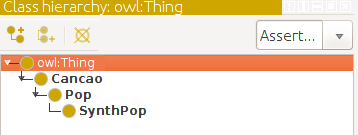
\includegraphics[width=0.5\textwidth]{Capitulos/Implementacao/ck1.png}
	\caption{As classes da ontologia de gêneros musicais.}
	\label{img:ck1}
\end{figure}

Com o comando abaixo, a operação é realizada. O resultado está na Figura \ref{img:ck2}.

\begin{small}
	\texttt{java -jar ontologyrepair-1.0.0-SNAPSHOT.jar -c --core-retainment -i cancao.owl \\ -o output.owl -f "SynthPop SubClassOf Pop"}
\end{small}

\begin{figure}[H]
	\centering
	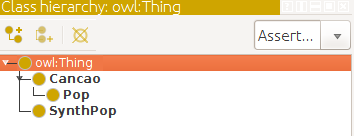
\includegraphics[width=0.5\textwidth]{Capitulos/Implementacao/ck2.png}
	\caption{O resultado da operação Contração \textit{Kernel}.}
	\label{img:ck2}
\end{figure}


\subsection{Contração \textit{Partial Meet}}

Para a contração \textit{Partial Meet}, o exemplo utilizado tem as classes \texttt{Musica}, \texttt{Cancao} e \texttt{HinoNacional}, e os seguintes axiomas: 

\begin{itemize}
	\item \texttt{HinoNacional} $ \sqsubseteq $ \texttt{Cancao}
	\item \texttt{Cancao} $ \sqsubseteq $ \texttt{Musica}
\end{itemize}

Sua representação fica como na Figura \ref{img:cpm1}.

\begin{figure}[H]
	\centering
	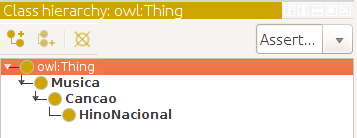
\includegraphics[width=0.5\textwidth]{Capitulos/Implementacao/cpm1.png}
	\caption{A estrutura da ontologia de tipos de música.}
	\label{img:cpm1}
\end{figure}

Como definido anteriormente, na verdade, \texttt{Cancao} e \texttt{HinoNacional} são classes na mesma hierarquia, portanto, precisamos remover \texttt{HinoNacional} $ \sqsubseteq $ \texttt{Cancao}. A operação é realizada com o seguinte comando:

\begin{small}
	\texttt{java -jar ontologyrepair-1.0.0-SNAPSHOT.jar -c --relevance -i musica.owl \\ -o output.owl -f "HinoNacional SubClassOf Cancao"}
\end{small}

Após a sua execução, acontece o desejado, mas aparentemente, esse não é o melhor resultado, como pode ser visto na Figura \ref{img:cpm2}.

\begin{figure}[H]
	\centering
	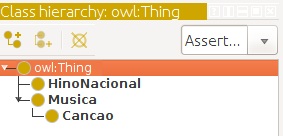
\includegraphics[width=0.5\textwidth]{Capitulos/Implementacao/cpm2.png}
	\caption{O resultado da operação Contração \textit{Partial Meet}.}
	\label{img:cpm2}
\end{figure}

\subsection{Revisão \textit{Kernel}}

O exemplo usado para a Revisão \textit{Kernel} será simples também. Sejam um fragmento da ontologia de música os axiomas abaixo e representação como na Figura \ref{img:r1}.

\begin{itemize}
	\item \texttt{FunkAmericano} $ \sqsubseteq $ \texttt{Cancao}
	\item \texttt{FunkBrasileiro} $ \sqsubseteq $ \texttt{FunkAmericano}
\end{itemize}

\begin{figure}[H]
	\centering
	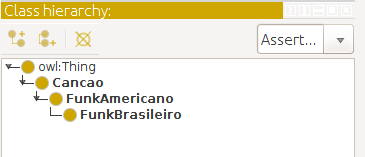
\includegraphics[width=0.5\textwidth]{Capitulos/Implementacao/r1.png}
	\caption{A estrutura da outra ontologia de gêneros musicais.}
	\label{img:r1}
\end{figure}

No entanto, hoje já se classifica o Funk Brasileiro como distinto do Funk Americano. Logo, vamos adicionar à nossa base que os dois subgêneros são disjuntos.

Com o comando abaixo, acontece a operação:

\begin{small}
	\texttt{java -jar ontologyrepair-1.0.0-SNAPSHOT.jar -r -i funk.owl -o output.owl \\ -f "FunkBrasileiro DisjointWith FunkAmericano"}
\end{small}

O resultado é visto abaixo. Note que a propriedade de disjunção está no produto final. Ambos os produtos podem ser observados na Figura \ref{img:r2}.

\begin{figure}[H]
	\centering
	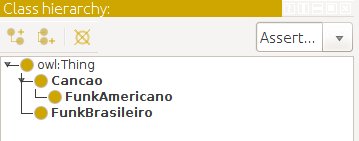
\includegraphics[width=0.45\textwidth]{Capitulos/Implementacao/r2.png}
	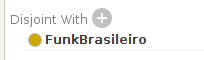
\includegraphics[width=0.45\textwidth]{Capitulos/Implementacao/r3.png}
	\caption{O resultado da operação Revisão \textit{Kernel} e a presença da disjunção, na classe \texttt{FunkAmericano}, respectivamente.}
	\label{img:r2}
\end{figure}

\subsection{Pseudocontração SRW}

Para a Pseudocontração SRW, serão consideradas as classes \texttt{Cantor} e \texttt{Compositor} da ontologia musical, e o seguinte axioma: \texttt{Compositor} $ \sqsubseteq $ \texttt{Cantor}, com a representação exibida na Figura \ref{img:srw1}.

\begin{figure}[H]
	\centering
	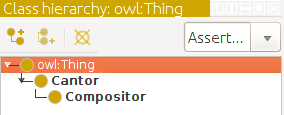
\includegraphics[width=0.5\textwidth]{Capitulos/Implementacao/srw1.png}
	\caption{A estrutura da ontologia sobre ocupações na área de música.}
	\label{img:srw1}
\end{figure}

Ela possui um indivíduo, \texttt{markRonson}, pertencente à classe \texttt{Compositor}, como se mostra na Figura \ref{img:srw2}.

\begin{figure}[H]
	\centering
	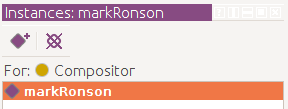
\includegraphics[width=0.5\textwidth]{Capitulos/Implementacao/srw2.png}
	\caption{A instância da ontologia.}
	\label{img:srw2}
\end{figure}

Tudo isso implica que \texttt{markRonson} também é um \texttt{Cantor}, o que está errado. 

A operação pode ser feita com o seguinte comando:

\begin{small}
	\texttt{java -jar ontologyrepair-1.0.0-SNAPSHOT.jar -srw -i pessoa.owl -o output.owl \\ -f "markRonson Type: Cantor"}
\end{small}

Depois da operação, temos que \texttt{Compositor} deixa de ser subclasse de \texttt{Cantor}, e então, \texttt{markRonson} não pertence mais à classe \texttt{Cantor}, como se observa na Figura \ref{img:srw3}.

\begin{figure}[H]
	\centering
	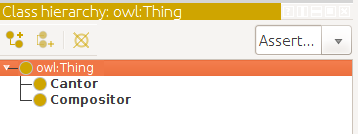
\includegraphics[width=0.5\textwidth]{Capitulos/Implementacao/srw3.png}
	\caption{O resultado da operação Pseudocontração SRW.}
	\label{img:srw3}
\end{figure}
